\documentclass[10pt,a4paper]{article}

% Đường dẫn từ thư mục meeting-01 đến assets/ của repository.
\newcommand{\HCMUTAssetPath}{../../../../assets}
\NeedsTeXFormat{LaTeX2e}
\ProvidesPackage{hcmut-report}[2026/09/10 Shared HCMUT report style]

\RequirePackage{fontspec}
\RequirePackage[a4paper,total={160mm,240mm},left=30mm,top=30mm]{geometry}
\RequirePackage{graphicx}
\RequirePackage{tikz}
\RequirePackage{fancyhdr}
\RequirePackage{lastpage}
\RequirePackage{caption}
\RequirePackage{tabularx}
\RequirePackage{longtable}
\RequirePackage{booktabs}
\RequirePackage{array}
\RequirePackage[table]{xcolor}
\RequirePackage{enumitem}
\RequirePackage{etoolbox}
\RequirePackage{setspace}
\RequirePackage[unicode,colorlinks=true,linkcolor=black,urlcolor=blue,citecolor=black]{hyperref}

% Latin Modern giữ gần phong cách Computer Modern/VnTeX của báo cáo tham khảo,
% đồng thời hiển thị tiếng Việt Unicode tốt khi biên dịch bằng XeLaTeX.
\setmainfont{lmroman10-regular.otf}[
  BoldFont=lmroman10-bold.otf,
  ItalicFont=lmroman10-italic.otf,
  BoldItalicFont=lmroman10-bolditalic.otf
]
\setmonofont{lmmono10-regular.otf}[
  BoldFont=lmmonolt10-bold.otf,
  ItalicFont=lmmonolt10-oblique.otf
]

\providecommand{\HCMUTAssetPath}{..}
\providecommand{\UniversityName}{ĐẠI HỌC QUỐC GIA THÀNH PHỐ HỒ CHÍ MINH}
\providecommand{\SchoolName}{TRƯỜNG ĐẠI HỌC BÁCH KHOA}
\providecommand{\FacultyName}{KHOA KHOA HỌC VÀ KỸ THUẬT MÁY TÍNH}
\providecommand{\ReportType}{BÁO CÁO}
\providecommand{\ReportTitle}{BÀI TẬP LỚN CÔNG NGHỆ PHẦN MỀM}
\providecommand{\ReportSubjectLabel}{ĐỀ TÀI:}
\providecommand{\ProjectTitle}{SMART E-MOBILITY HUB}
\providecommand{\ProjectSubtitle}{}
\providecommand{\CourseCode}{CO3001}
\providecommand{\LecturerName}{}
\providecommand{\ClassCode}{}
\providecommand{\Semester}{Học KỲ 261}
\providecommand{\AcademicYear}{2026 -- 2027}
\providecommand{\PlaceAndDate}{TP. Hồ Chí Minh, tháng 09/2026}
\providecommand{\FooterTitle}{Bài tập lớn Công nghệ phần mềm}
\providecommand{\CoverReportTypeStyle}{\LARGE\bfseries}
\providecommand{\CoverReportTitleStyle}{\Large\bfseries}
\providecommand{\CoverSubjectLabelStyle}{\large\bfseries}
\providecommand{\CoverProjectTitleStyle}{\Large\bfseries}
\providecommand{\CoverProjectSubtitleStyle}{\large\bfseries}

\setlength{\headheight}{40pt}
\setlength{\parindent}{1.25cm}
\setlength{\parskip}{2pt}
\setstretch{1.15}
\setlist{nosep,leftmargin=1.8em}
\setcounter{secnumdepth}{3}
\setcounter{tocdepth}{2}

\renewcommand{\thesection}{\Roman{section}}
\renewcommand{\thesubsection}{\arabic{subsection}}
\renewcommand{\thesubsubsection}{\arabic{subsection}.\arabic{subsubsection}}

\renewcommand{\figurename}{Hình}
\renewcommand{\tablename}{Bảng}
\renewcommand{\contentsname}{MỤC LỤC}
\renewcommand{\listfigurename}{DANH SÁCH HÌNH}
\renewcommand{\listtablename}{DANH SÁCH BẢNG}
\captionsetup{
  font=small,
  labelfont=bf,
  textfont=it,
  labelsep=colon,
  justification=centering,
  singlelinecheck=true
}
\captionsetup[figure]{aboveskip=6pt,belowskip=2pt}
\captionsetup[table]{aboveskip=6pt,belowskip=2pt}

\newcolumntype{Y}{>{\raggedright\arraybackslash}X}
\newcolumntype{C}[1]{>{\centering\arraybackslash}p{#1}}
\newcolumntype{L}[1]{>{\raggedright\arraybackslash}p{#1}}
\renewcommand{\arraystretch}{1.25}
\arrayrulecolor{black}

\pagestyle{fancy}
\fancyhf{}
\fancyhead[L]{%
  \begin{tabular}{@{}c@{\hspace{2mm}}l@{}}
    
\includegraphics[width=8mm,height=8mm]{\HCMUTAssetPath/hcmut (1).png} &
    \begin{tabular}{@{}l@{}}
      \scriptsize\bfseries\ttfamily Trường Đại Học Bách Khoa -- ĐHQG TP.HCM\\[-1pt]
      \scriptsize\bfseries\ttfamily Khoa Khoa học và Kỹ thuật Máy tính
    \end{tabular}
  \end{tabular}%
}
\fancyfoot[L]{\scriptsize\ttfamily \FooterTitle\\Niên khoá \AcademicYear}
\fancyfoot[R]{\scriptsize\ttfamily Trang \thepage/\pageref*{LastPage}}
\renewcommand{\headrulewidth}{0.3pt}
\renewcommand{\footrulewidth}{0.3pt}

\newcommand{\MakeHCMUTCover}{%
  \hypersetup{pageanchor=false}%
  \begin{titlepage}
    \thispagestyle{empty}
    \begin{tikzpicture}[remember picture,overlay,inner sep=0,outer sep=0]
      \coordinate (A) at ([xshift=-15mm,yshift=-20mm]current page.north east);
      \coordinate (B) at ([xshift=24mm,yshift=-20mm]current page.north west);
      \coordinate (C) at ([xshift=24mm,yshift=20mm]current page.south west);
      \coordinate (D) at ([xshift=-15mm,yshift=20mm]current page.south east);
      \draw[blue!80!black,line width=4pt] (A)--(B)--(C)--(D)--cycle;
      \draw[line width=0.35pt]
        ([yshift=5mm,xshift=-5mm]A)--([yshift=5mm,xshift=5mm]B)--
        ([yshift=-5mm,xshift=5mm]B)--([yshift=-5mm,xshift=-5mm]B)--
        ([yshift=5mm,xshift=-5mm]C)--([yshift=5mm,xshift=5mm]C)--
        ([yshift=-5mm,xshift=5mm]C)--([yshift=-5mm,xshift=-5mm]D)--
        ([yshift=5mm,xshift=-5mm]D)--([yshift=5mm,xshift=5mm]D)--
        ([yshift=-5mm,xshift=5mm]A)--([yshift=-5mm,xshift=-5mm]A)--
        ([yshift=5mm,xshift=-5mm]A);
      \draw[line width=0.35pt]
        ([yshift=-3mm,xshift=3mm]A)--([yshift=-3mm,xshift=-3mm]B)--
        ([yshift=3mm,xshift=-3mm]B)--([yshift=3mm,xshift=3mm]B)--
        ([yshift=-3mm,xshift=3mm]C)--([yshift=-3mm,xshift=-3mm]C)--
        ([yshift=3mm,xshift=-3mm]C)--([yshift=3mm,xshift=3mm]D)--
        ([yshift=-3mm,xshift=3mm]D)--([yshift=-3mm,xshift=-3mm]D)--
        ([yshift=3mm,xshift=-3mm]A)--([yshift=3mm,xshift=3mm]A)--
        ([yshift=-3mm,xshift=3mm]A);
    \end{tikzpicture}

    \begin{center}
      \vspace*{-7mm}
      {\large \UniversityName\par}
      \vspace{1mm}
      {\large \SchoolName\par}
      \vspace{1mm}
      {\large\bfseries \FacultyName\par}

      \vspace{10mm}
      
\includegraphics[width=44mm]{\HCMUTAssetPath/logo BK.png}

      \vspace{10mm}
      {\CoverReportTypeStyle \ReportType\par}
      \vspace{3mm}
      {\CoverReportTitleStyle \ReportTitle\par}

      \vspace{10mm}
      \ifdefempty{\ReportSubjectLabel}{}{%
        {\CoverSubjectLabelStyle \ReportSubjectLabel\par}\vspace{3mm}%
      }
      {\CoverProjectTitleStyle \ProjectTitle\par}
      \ifdefempty{\ProjectSubtitle}{}{%
        \vspace{3mm}{\begin{minipage}{0.84\textwidth}\centering\CoverProjectSubtitleStyle \ProjectSubtitle\end{minipage}\par}%
      }

      \vfill
      \begin{tabular}{@{}rl@{}}
        \textbf{Mã môn học:} & \CourseCode\\[2mm]
        \textbf{Giảng viên hướng dẫn:} & \LecturerName\\[2mm]
        \ifdefempty{\ClassCode}{}{\textbf{Lớp:} & \ClassCode\\[2mm]}
        \textbf{Học kỳ:} & \Semester
      \end{tabular}

      \vfill
      {\large \PlaceAndDate\par}
      \vspace*{9mm}
    \end{center}
  \end{titlepage}
  \clearpage
  \pagenumbering{arabic}
  \hypersetup{pageanchor=true}%
}

\newenvironment{HCMUTMemberTable}{%
  \begin{longtable}{|C{10mm}|L{45mm}|C{27mm}|L{50mm}|}
    \hline
    \rowcolor{gray!15}
    \textbf{STT} & \centering\arraybackslash\textbf{Họ và tên} &
    \textbf{MSSV} & \centering\arraybackslash\textbf{Vai trò / Nhiệm vụ}\\
    \hline
    \endfirsthead
    \hline
    \rowcolor{gray!15}
    \textbf{STT} & \centering\arraybackslash\textbf{Họ và tên} &
    \textbf{MSSV} & \centering\arraybackslash\textbf{Vai trò / Nhiệm vụ}\\
    \hline
    \endhead
}{%
  \end{longtable}
  \addtocounter{table}{-1}
}

\newcommand{\MemberRow}[4]{#1 & #2 & #3 & #4\\\hline}

% Thông tin riêng của biên bản họp buổi 01.
\renewcommand{\ReportType}{BIÊN BẢN HỌP NHÓM}
\renewcommand{\ReportTitle}{CÔNG NGHỆ PHẦN MỀM}
\renewcommand{\ReportSubjectLabel}{}
\renewcommand{\ProjectTitle}{PHASE 1 -- BUỔI 01}
\renewcommand{\ProjectSubtitle}{TÌM HIỂU ĐỀ TÀI VÀ KIẾN THỨC NỀN}
\renewcommand{\CourseCode}{CO3001}
\renewcommand{\LecturerName}{Cô Trần Thị Ngọc Trâm}
\renewcommand{\ClassCode}{}
\renewcommand{\Semester}{Học kỳ 261}
\renewcommand{\AcademicYear}{2026 -- 2027}
\renewcommand{\PlaceAndDate}{TP. Hồ Chí Minh, ngày 07 tháng 09 năm 2026}
\renewcommand{\FooterTitle}{Biên bản họp nhóm -- Phase 1}


\begin{document}

\pagenumbering{gobble}
\MakeHCMUTCover

\section{THÔNG TIN BUỔI HỌP}

\begin{table}[htbp]
  \centering
  \begin{tabularx}{\textwidth}{|>{\bfseries}L{45mm}|Y|}
    \hline
    Lần họp & Buổi 01 -- Phase 1\\
    \hline
    Ngày họp & 07/09/2026\\
    \hline
    Thời gian bắt đầu & 20:30\\
    \hline
    Chủ đề & Tìm hiểu đề tài Smart E-Mobility Hub và kiến thức nền cho Phase 1\\
    \hline
    Giảng viên hướng dẫn & Cô: Trần Thị Ngọc Trâm\\
    \hline
    Người chủ trì & Trần Nhật Bảo Anh -- Nhóm trưởng\\
    \hline
  \end{tabularx}
\end{table}

\section{THÀNH PHẦN NHÓM}

\begin{HCMUTMemberTable}
  \MemberRow{1}{Nguyễn Quốc Trung}{2413707}{Thành viên}
  \MemberRow{2}{Phan Võ Bảo Trâm}{2413576}{Thành viên}
  \MemberRow{3}{Lê Nguyễn Tường Vi}{2413937}{Thành viên}
  \MemberRow{4}{Nguyễn Ngọc Hân}{2410951}{Thành viên}
  \MemberRow{5}{Trần Thị Hương Giang}{2410845}{Thành viên}
  \MemberRow{6}{Nguyễn Thị Minh Anh}{2410126}{Thành viên}
  \MemberRow{7}{Trần Nhật Bảo Anh}{2410155}{Nhóm trưởng}
\end{HCMUTMemberTable}

\noindent Buổi họp có sự tham gia của đầy đủ bảy thành viên trong nhóm.

\section{MỤC TIÊU BUỔI HỌP}

\begin{itemize}
  \item Cùng đọc và thống nhất cách hiểu ban đầu về đề tài Smart E-Mobility Hub.
  \item Nhận diện các nhóm người dùng, tài nguyên và quy trình nghiệp vụ chính của hệ thống.
  \item Tìm hiểu những khái niệm Công nghệ phần mềm cần dùng trước khi viết nội dung Phase 1.
  \item Ghi lại các điểm chưa rõ trong đề bài để trao đổi với giảng viên trước khi phân công công việc.
\end{itemize}

\section{NỘI DUNG THẢO LUẬN}

\subsection{Cách hiểu ban đầu về đề tài}

Nhóm hiểu Smart E-Mobility Hub là hệ thống hỗ trợ quản lý và điều phối phương tiện điện trong Khu đô thị ĐHQG-HCM. Hệ thống phải quản lý các Hub, phương tiện dùng chung, vị trí đỗ, cổng sạc và trạng thái sử dụng của từng tài nguyên.

Từ nội dung đề bài, nhóm xác định ba nhóm tình huống chính cần tiếp tục phân tích:

\begin{itemize}
  \item Sinh viên tìm kiếm, đặt, nhận và trả phương tiện dùng chung.
  \item Người dùng xe điện cá nhân đặt chỗ đỗ hoặc đăng ký sạc.
  \item Đơn vị vận hành theo dõi toàn mạng lưới, xử lý sự cố, điều phối tài nguyên và thực hiện mô phỏng What-if.
\end{itemize}

Nhóm nhận thấy trọng tâm của bài toán nằm ở việc quản lý trạng thái và phân bổ các tài nguyên có giới hạn. Buổi họp đầu tiên chưa đi sâu vào công nghệ triển khai, framework hoặc thiết kế cơ sở dữ liệu.

\subsection{Kiến thức nền đã cùng tìm hiểu}

\begin{itemize}
  \item \textbf{Quy trình phát triển phần mềm:} yêu cầu ở Phase 1 là cơ sở cho mockup, behavioral diagram, kiến trúc, thiết kế lớp, kiểm thử và MVP trong các phase sau.
  \item \textbf{Stakeholder và actor:} stakeholder là cá nhân hoặc đơn vị có lợi ích liên quan; actor là vai trò tương tác trực tiếp với hệ thống.
  \item \textbf{Phạm vi và ranh giới hệ thống:} cần phân biệt chức năng thuộc phần mềm với công việc do con người, thiết bị hoặc hệ thống bên ngoài thực hiện.
  \item \textbf{Các loại yêu cầu:} functional requirement mô tả hệ thống phải làm gì; business rule nêu quy tắc nghiệp vụ; non-functional requirement quy định chất lượng và ràng buộc của hệ thống.
  \item \textbf{Use case:} use-case diagram cho biết actor nào sử dụng chức năng nào; use-case specification mô tả chi tiết luồng chính, luồng thay thế, tiền điều kiện và hậu điều kiện. Nhóm mới dừng ở mức làm quen, chưa vẽ diagram trong buổi này.
\end{itemize}

\subsection{Những nội dung chưa rõ}

Sau khi đọc đề, nhóm thống nhất cần hỏi lại giảng viên các vấn đề sau:

\begin{enumerate}
  \item Phần group work và individual work sẽ do ai nộp, nộp bao nhiêu file và hai phần được phép trùng nội dung ở mức nào.
  \item Biên bản họp cần lập theo từng tuần hay từng phase, gồm những mục bắt buộc nào và được nộp kèm theo phần nào của báo cáo.
  \item Phần công khai sử dụng Generative AI có bắt buộc cung cấp prompt hay không, và cần mô tả phần chỉnh sửa, phát triển thêm của nhóm đến mức nào.
  \item What-if Simulation cần được phân tích chi tiết ngay từ Phase 1 hay chỉ cần xác định như một nhóm chức năng.
  \item Phạm vi hợp lý của MVP và ranh giới giữa nội dung làm chung với nội dung mỗi thành viên phải tự thực hiện.
\end{enumerate}

\section{KẾT LUẬN BUỔI HỌP}

\begin{itemize}
  \item Nhóm đã có cách hiểu chung ban đầu về bài toán, các đối tượng nghiệp vụ và mục tiêu của hệ thống.
  \item Kiến thức nền mới ở mức làm quen. Nhóm cần tiếp tục đọc đề và thống nhất thuật ngữ trước khi viết yêu cầu chính thức.
  \item Các yêu cầu về hình thức nộp bài, biên bản họp, minh chứng sử dụng AI và phạm vi sản phẩm vẫn cần được giảng viên xác nhận.
  \item Nhóm chưa phân công nhiệm vụ Phase 1 trong buổi họp này.
\end{itemize}

\section{CÔNG VIỆC SAU BUỔI HỌP}

Tại thời điểm kết thúc buổi họp, nhóm \textbf{chưa giao đầu việc riêng cho bất kỳ thành viên nào}. Cả nhóm tiếp tục đọc đề bài và ghi lại các điểm chưa rõ. Nhóm trưởng sẽ tổng hợp câu hỏi để trao đổi với giảng viên. Việc phân công chính thức sẽ được thực hiện sau khi nhóm nhận được phản hồi và chốt phạm vi Phase 1.

\begin{samepage}
\noindent Nội dung dự kiến cho buổi họp tiếp theo:

\begin{itemize}
  \item Tổng hợp câu trả lời của giảng viên cho các vấn đề còn chưa rõ.
  \item Chốt phạm vi và danh sách sản phẩm cần hoàn thành trong Phase 1.
  \item Thống nhất cách viết, quy ước đặt mã requirement và cách quản lý phiên bản tài liệu.
  \item Phân công công việc cho bảy thành viên và thống nhất thời hạn nội bộ.
\end{itemize}
\end{samepage}

\end{document}
